
{\color{blue}3-10: We continue the 2D Ising model. Much of what we say will hold true for other planar graphs. }

The energy is 
\be
\sum_{b\in \mathcal{E}}J_b (\sigma\sigma)_b - h\sum_{x\in G}\sigma_x
\ee 
where the first sum is over edges (bonds) and if $b=b_1b_2$, then $(\sigma\sum_{n=0}^{\infty})_b$ denotes $\sigma_{b_1}\sigma_{b_2}$.

The state changes discontinuously across the line $h=0$ until some critical temperature $T_c$. Along the symmetry line the model is solvable.
\begin{theorem}[Onsager]
For the nn $\mathbb{Z}^2$ at $h=0$, $J_b=J$, 
\be
\frac{1}{|\Lambda|} \ln Z_{\Lambda}^{\text{per}} (\beta, 0) = \ln \cosh (\beta J)
+ \frac{1}{2} \int_{(-\pi, \pi]^2} \frac{dx_1\,dx_2}{(2\pi)^2}\ln \left\{ {
\left[ {
Y(\beta) + Y^{-1}(\beta) - 2
} \right] + \mathcal{E}(k)
} \right\}
\ee
where $\mathcal{E}(k) = 2\left[ {\sin^2 \left( {\frac{k_1}{2}} \right) + \sin^2\left( {\frac{k_2}{2}} \right)} \right]$.

By the integral we really mean the discrete sum over $k\in (-\pi,\pi]^2 \cap \frac{2\pi}{L}\mathbb{Z}^2$. (In the infinite volume limit it is an integral.)
%elastic membrane.
\end{theorem}
%discrete momenta as sites in spce.
For square summable function in a box, we can look at a basis of delta functions, or the Fourier basis $e^{ik\cdot x}$ for $k\in (-\pi,\pi]^2 \cap \frac{2\pi}{L}\mathbb{Z}^2$. I.e., $k$ is sampled from the dual lattice; $[-\pi,\pi]$ is subdivided to have the right number of points.
%condensed matter physics. Fourier analysis.
%In many books where Onsager's theorem..., they stop short of this expression.

Note $\sinh$ is an unbounded monotone increasing function. 
%what $Y+Y^{-2}-2$ looks like: min 0 at 1.
%sum won't be both 0 if temperature is other than 0.
%At the critical temperature, $Y(\be)+Y^{-1}(\be)-2$ vanishes, and the singularities are those of $\cal E(k)$.

For $h=0, b\in \mathcal{E}(\mathcal{G})$,
\begin{align*}
Z_{\Lambda} &= \frac{1}{2^{|\Lambda|}} \sum_{\sigma \in \Omega_{\Lambda}} e^{-\beta H_{\Lambda}(\sigma)}\\
&\qquad e^{-\beta H(\sigma)} = e^{\sum_b (\sigma\sigma)_b \beta J_b} = \prod_b e^{\beta J_b (\sigma\sigma)_b}& \text{(factorizing over bonds)}\\
&=\frac{1}{2^{|\Lambda|}} \sum_{\sigma\in \Omega_{\Lambda}} \prod_b [\cosh(\beta J_b) + \sinh(\beta J_b)(\sigma\sigma)_b]&e^x = \cosh x + \sinh x\\
&=\left[ {\prod_b \cosh(\beta J_b)} \right] \frac{1}{2^{|\Lambda|}}\sum_{\sigma\in \Omega_{\Lambda}} \prod_b[1+K_b(\sigma\sigma)_b]&\text{where }K_b=\tanh(\beta J_b)\\
&=\left[ {\prod_b \cosh(\beta J_b)} \right] \mathop{\mathbb E}_{\sigma} \sum_{\Gamma\subseteq \mathcal{E}(\mathcal{G})}\prod_{b\in \Gamma}K_b \left( {\prod_{b=\{x,y\}\text{ in }\Gamma} (\sigma\sigma)_b} \right)\\ 
&=\left[ {\prod_b \cosh(\beta J_b)} \right] \sum_{\Gamma}\prod_{b\in \Gamma}K_b
\mathop{\mathbb E}_{\sigma} \left( {\prod_{b=\{x,y\}\text{ in }\Gamma} (\sigma\sigma)_b} \right)&\text{linearity of expectation}
\end{align*}
We expressed the sum in terms of the symmetric and anti-symmetric parts and pulled out a factor $\cosh$. 
%\fixme{Where $\Ga$...}
%Here $\Ga$ is over sets of loops (i.e., possibilities for the places where $(\si\si)_b=-1$).
%nmber of bonds contain a site x
%if single side for which this is an odd poewr, the average is 0.
%if the power is even for all spins, the averge is 1.
The average is easy to compute: if there is a spin for which the power is odd, the average is 0; if the power is even for all spins, the average is 1.
\be
\mathop{\mathbb E}_{\sigma} \left( {\prod_{b\in \Gamma} (\sigma\sigma)_b} \right) = \mathop{\mathbb E}_{\sigma}\prod_x \sigma_x^{\sum_{b\in \Gamma} \mathds{1} [b\ni x]}
= \mathds{1}[\forall x,(-1)^{\sum_{b\in \Gamma} \mathds{1}[b\ni x]}=1]
\ee
%good graph obtained from closing

%Factorize over bonds
%\bal
%e^{-\be H(\si)} &= e^{\sum_b (\si\si)_b \be J_b} = \prod_b e^{\be J_b (\si\si)_b}.
%\end{align*}
Let $(\partial \Gamma)_2=\left\{{x}:{x\text{ belongs to an odd number of edges}}\right\}$. The condition for the summand to not vanish is $(\partial \Gamma)_2=\phi$.

We summarize this calculation as a lemma.

%\begin{theorem}[Feynman-Sherman]
%
%\end{theorem}
%complexity not reduced yet.
\begin{lemma}
For $h=0$,
\begin{align*}
Z_\Lambda &= \left[ {\prod_b \cosh(\beta J_b)} \right] \sum_{\Gamma, (\partial \Gamma)_2=\phi} \prod_{b\in \Gamma}K_b.
\end{align*}
\end{lemma}

\begin{theorem}[Feynman-Sherman]
Let $K(\Lambda)= \prod_{b\in \Gamma} K_b$.
\be
\sum_{\Gamma:(\partial \Gamma)_2=\phi} K(\Gamma) =  \prod_{\text{loops}}[1+(-1)^{n(l)}K(l)]
\ee
where $n(l)$ is the number of self-intersections of $l$.
\end{theorem}
Each graph can be covered by a collection of loops (which can cross and repeat edges).
%completing loops
%start from RHS: double counting.
Note the RHS is an infinite sum. By a lot of identities this infinite sum reduces to a finite sum.

Kac-Ward introduced the Ihara zeta function.

The RHS is 
\begin{align*}
 \prod_{\text{loops}}[1+(-1)^{n(l)}K(l)] &= \sum_{m:\mathcal{E}(G) \to \mathbb{Z}_+} {\prod_b K_b^{m_b}} W(m)\\
\text{where }W(m) &= \sum_{\ell_1,\ldots} \prod_j (-1)^{n_{\ell_j}}\mathds{1}_m[\{\ell_1,\ldots, \ell_k\}].
\end{align*}

%how many times is each bond is visited by each loop of collection...
%when weights small enough, convergent infinite product
%how many ways edge is visited.

\begin{lemma}
If $\left\Vert {m}\right\Vert_{\infty}:=\max_b(m_b)=1$ then $W(m)=1$.
\end{lemma}
%If weights are 0 or 1 for all bonds, then the contribution of the RHS is 1. Sticking just with $W(m)=1$, this captures all partition functions.

Sum over the multisets of edges. We need to enumerate how many ways the multisets can be realized as a union of loops. 
The Katz-Ward idea is enumerate all the different ways to resolve the traffic jams at each vertex with an intersection: sum over all possible choices with the right signs. The other vertices don't present any choices for the prospective loop.

\begin{center}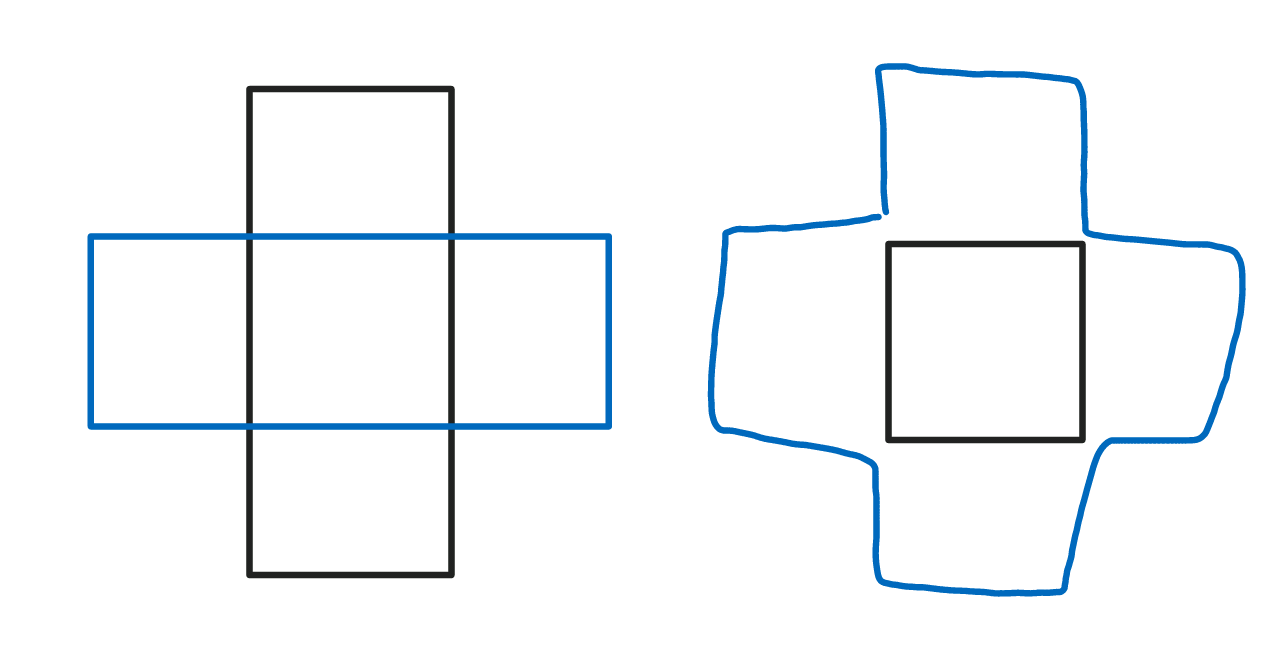
\includegraphics[scale=.25]{images/12-2}\end{center}

The three possibilities are:

\begin{center}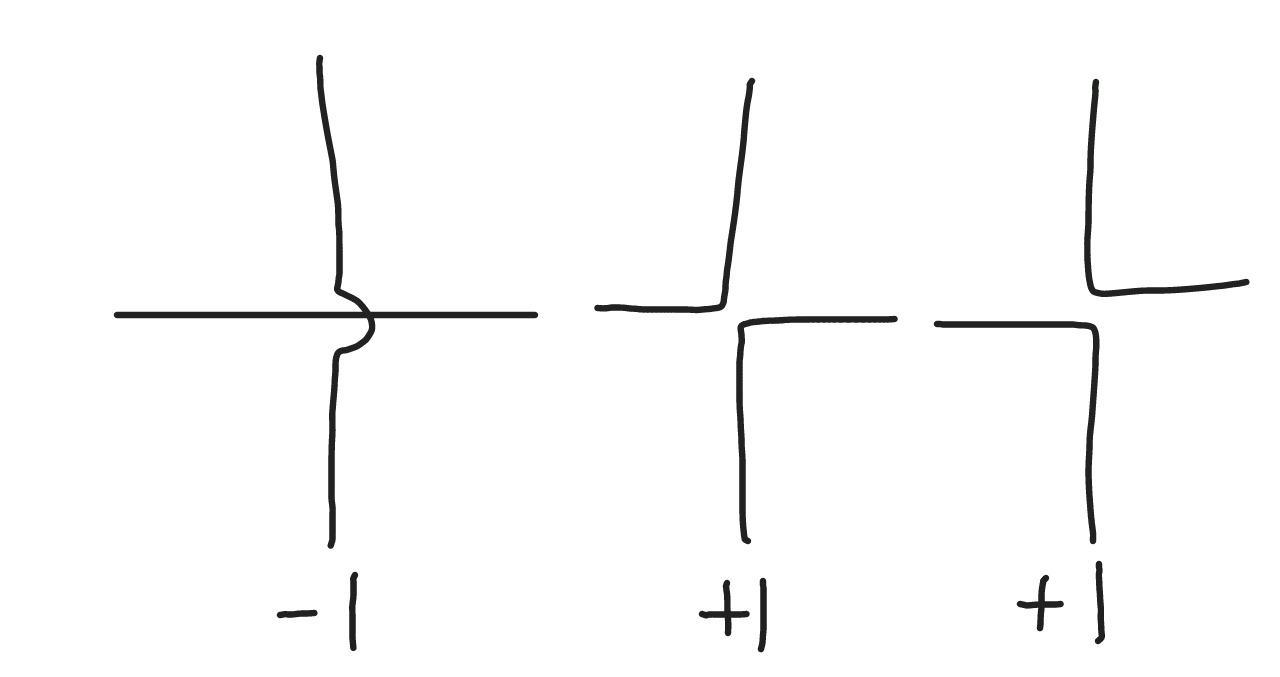
\includegraphics[scale=.25]{images/12-3}\end{center}

%The sum is 1.
%Think of loops as limits of continuous curves. It's not clear whether under magnification... the number of times curves cross each other.
The parity is certain. 
%the number of crossings disappear from view.
%deformation: disentangle wire.
%Whitney theorem. Intuitive things hard to prove.
%crossing of single curve with self or other. 
%Two curves always have an even number of intersections. (If you pull them apart, intersections will disappear in pairs.)

\begin{lemma}
If $\left\Vert {m}\right\Vert_{\infty}=2$ then $W=0$.
\end{lemma}
\begin{proof}
This means there is one edge traversed twice. Take one of these edges. How are the loops arranged in the complement? There are 2 possibilities for how the loops hook up through the bond. Summing you get 0.
\end{proof}
What if it's $>2$? This is in fact true for any value $>1$.

Why are the higher powers 0? %There are things like graph zeta functions.

\begin{theorem}[Sherman]\label{thm:sherman} %Kac-Wald, 
\be
\prod_{\text{loops}} [1+(-1)^{n(\ell)}K(\ell)]^2 = \det(\mathds{1} - \mathcal{L})
\ee
where $\mathcal{L}$ is a $2|\mathcal{E}|\times 2|\mathcal{E}|$ matrix indexed by the oriented edges. Here 
\be
\mathcal{L}_{e,e'} = \delta_{O(e'),t(e)} e^{\frac{i\angle(e,e')}{2}}K_e.
%$e$ to flow into $e'$.
\ee
(The Kronecker delta function says that $e$ has to flow into $e'$, i.e., the terminal of $e$ is the same as the origin of $e'$. Here $\angle(e,e')$ means the angle between $e,e'$. We get a phase number that's half the sum of the turns. For a simple loop, we get $-1$.)
\end{theorem}
$\text{Tr} \mathcal{L}^n = \sum_{e_1,\ldots, e_n} = \mathcal{L}_{e_1,e_n}\cdots \mathcal{L}_{e_2,e_1}$. This is associated to an oriented loop.
%n(\ell)$ self intersections.

%There's a general relation...
%Finite product expression for infinite product.
Buried in this is an infinite collection of relations. In principle we have contributions in the RHS of the theorem with arbitrarily many loops. But Sherman's theorem says that it is multilinear in the weights of the edges. Higher powers do not contribute. 

You can decompose the Hilbert space into Fourier modes. For each value of the momentum you have a finite-dimensional space. Edges are indexed by position and direction. If you change to momenta and direction, the different momenta are not mixed by shifting. The determinant is a block determinant where different values of the momenta are not mixed. We get $4\times 4$ blocks; the determinants can be computed and we get the solution.